\begin{tikzpicture}
  \matrix[ampersand replacement=\&]
  {
    \node (i1) {
    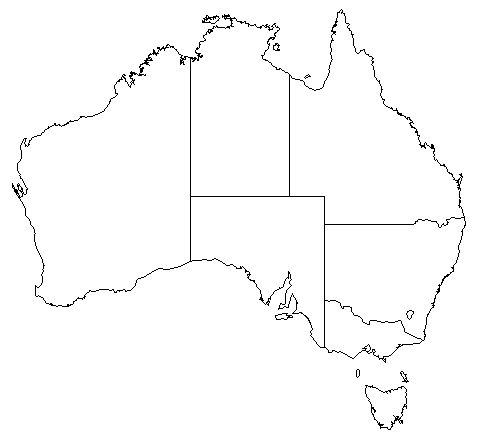
\includegraphics[width=.2\textwidth]{australia.pdf}}; \&[2mm]  
    \node(i2){
    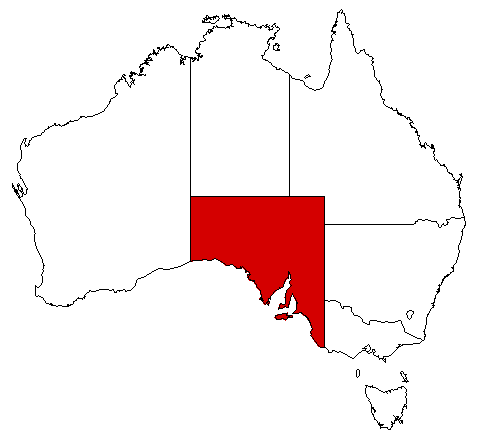
\includegraphics[width=.2\textwidth]{st-red.pdf}}; \&[2mm]
    \node(i3){
    
\includegraphics[width=.2\textwidth]{st-red-ql-blue.pdf}}; \&[2mm]
	\node(i4){
    
\includegraphics[width=.2\textwidth]{st-red-ql-blue-nt-green.pdf}};
    \\ 
	\node (l1) {Alle unbelegt}; \& 
	\node (l2) {SA in 5 Constraints}; \&
	\node(l3){$|D_\mathsf{QL}|$ nur 2 }; \&	
	\node(l4){$|D_\mathsf{NT}|$ nur 1 }; \&	
		
	\\
  };
  
\end{tikzpicture}